%=====================================
% Author: Christian Fischer Pedersen
% About: Slide template
%=====================================
%==============================
%   Author: Christian Fischer Pedersen
%   About: Beamer style file
%==============================

%========General
\documentclass[compress,mathserif,presentation,notheorems]{beamer}
%\usepackage[export]{adjustbox}
\usepackage{etex}
\usepackage[utf8]{inputenc}%Danske bogstaver
\usetheme{default}
\usecolortheme{default}

%========Fonts
\setbeamercolor{structure}{fg=aaudblue}
\setbeamerfont{structure}{family=\sf\bfseries}
\setbeamercolor{normal text}{fg=black}
\setbeamerfont{normal text}{family=\sf\mdseries}
\renewcommand{\footnoterule}{}
\renewcommand{\footnotesize}{\tiny}

%========Sections
\AtBeginSection[]{\begin{frame}\frametitle{Outline}\tableofcontents[currentsection]\end{frame}}

%========Parts
\makeatletter
\AtBeginPart{%
  \addtocontents{toc}{\protect\beamer@partintoc{\the\c@part}{\beamer@partnameshort}{\the\c@page}}%
}
%% number, shortname, page.
\providecommand\beamer@partintoc[3]{%
  \ifnum\c@tocdepth=-1\relax
    % requesting onlyparts.
    \sf{\bf{\textcolor{aaudblue}{\makebox[6em]{PART #1:}#2}}}
    \par
  \fi
}
\define@key{beamertoc}{onlyparts}[]{%
  \c@tocdepth=-1\relax
}
\makeatother

%========Itemize and enumerate
\setbeamertemplate{itemize items}[triangle]%triangle,circle,ball,square
\setbeamertemplate{note page}[plain]

%========Colors
\usepackage{pstricks,pst-node}
\newrgbcolor{aaudblue}{0.2 0.4 0.6}   %dark blue
\newrgbcolor{aaulblue}{0.4 0.6 0.8}   %light blue
\newrgbcolor{lgray}   {0.9 0.9 0.9} %light gray
\definecolor{lgray}{rgb}{0.9,0.9,0.9} %light gray
\definecolor{mgray}{rgb}{0.5,0.5,0.5} %medium gray
\definecolor{dgray}{rgb}{0.2,0.2,0.2} %dark gray

%========Footer
\beamertemplatenavigationsymbolsempty
\usepackage{tabularx}
\setbeamertemplate{footline}{
%\colorbox{white}
{\color{aaudblue}
\begin{tabularx}{0.98\textwidth}{l X}
~\insertshortauthor, \insertshortinstitute & \hfill \insertframenumber$|$\inserttotalframenumber\\
\end{tabularx}
}\vskip6pt
}

%========Header
\setbeamercolor*{palette tertiary}{fg=aaudblue,bg=white}
\setbeamertemplate{headline}{%
\begin{beamercolorbox}{section in head/foot}
\vskip6pt \insertsectionnavigationhorizontal{\paperwidth}{}{} \vskip2pt
%\vskip6pt \insertnavigation{\paperwidth} \vskip2pt
\end{beamercolorbox}%
}

%========Title page
\newcommand{\slidetitlepage}[2]{
\title{#1}
\subtitle{#2}
\author[Christian Fischer Pedersen]%
{Christian Fischer Pedersen\\[-1.4mm]%
%{\scriptsize Associate Professor, PhD}\\[-1.4mm]%
{\scriptsize cfp@eng.au.dk}}
\institute[Electrical and Computer Engineering, Aarhus University]%
{Section of Electrical and Computer Engineering\\
Department of Engineering\\
Aarhus University}
\date{{\scriptsize Revised on \today}}
}


%========Math fonts 
\usepackage{amsmath}
\usepackage{bbm}
\usepackage{pifont}
\usepackage{wasysym}
\usepackage{amssymb}
\usepackage{amsbsy}


%========Blocks
\setbeamertemplate{blocks}[rounded][shadow=true]
\setbeamercolor{block title} {bg=aaulblue,fg=white}
\setbeamercolor{block body}{bg=white,fg=black}%fg=lgray}

%========Figures and graphics
\usepackage[dvips]{epsfig}
\usepackage[dvips]{graphicx}
\usepackage{subfigure}
\usepackage{caption}%Skal komme efter 'subfigure' for ogsaa at virke paa denne
\usepackage{fancybox}\cornersize{1}
\usepackage{tikz}


%========Video and sound
%\usepackage{multimedia}


%========Tables
%\usepackage{booktabs}
\usepackage{rotating}
\usepackage{multirow}


%========Referencing and citations
\usepackage[sort&compress, numbers]{natbib}
\newcommand{\citefont}[1]%
{\fontsize{5pt}{5pt}\selectfont#1\normalsize}

\newcommand{\scite}[1]%Formerly known as "slidecite"
{\fontsize{5pt}{5pt}\selectfont(\citeauthor{#1}, \citeyear{#1} [\citenum{#1}])\normalsize}

\newcommand{\sciten}[1]%Formerly known as "slidecitenormal"
{(\citeauthor{#1}, \citeyear{#1} [\citenum{#1}])}

\newcommand{\scitennp}[1]%Formerly known as "slidecitenormalnp" - np means no parantheses 
{\citeauthor{#1}, \citeyear{#1} [\citenum{#1}]}

\newcommand{\scitesub}[1]%Formerly known as "slidecitesubmitted"
{\fontsize{5pt}{5pt}\selectfont(\citet{#1})\normalsize}

\renewcommand{\bibsection}{\subsubsection*{\bibname}} %Avoid 'References' in header

\newcommand{\shref}[2]%
{\href{#1}{\textcolor{aaudblue}{\textbf{#2}}}}

%\bibpunct[:]{(}{)}{;}{a}{}{,}

%========Misc. defines
\newcommand{\nolinefrac}[2]{\genfrac{}{}{0pt}{}{#1}{#2}}
\def\simiid{\overset{\scriptsize{i.i.d.}}{\sim}}
\def\CSMfac{$\textrm{CSM}_{\textrm{fac}}~$}
\def\CSMfft{$\textrm{CSM}_{\textrm{fft}}~$}
\def\Matlab{Matlab$^\copyright~$}
\def\rhoot{\mbox{\large{$\varrho$}}}

%========Vectors and matrices
\def\lambdav{\boldsymbol{\lambda}}
\def\lambdam{\mathbf{\Lambda}}
%\newcommand{\tlv}[1]{\tilde{\lv}^{{\raisebox{-2pt}{\footnotesize $(#1)$}}}} 
\def\deltav{\boldsymbol{\delta}}
\def\deltam{\mathbf{\Delta}}

%========Listings
\usepackage{listings}
% \lstset{
% nputencoding=T1,
% language=Matlab,
% xleftmargin=8pt,
% tabsize=2,
% basicstyle=\small, print whole listing small
% keywordstyle=\color{black}\bfseries, 
% identifierstyle=, nothing happens
% commentstyle=\color{black}\itshape,
% stringstyle=\color{black}\ttfamily,
% showstringspaces=false,
% numbers=left,
% stepnumber=0,
% numbersep=4pt,
% morekeywords={display}
% }

%Theorem environments
%----------------------------------------------------------
\usepackage{amsthm}
\theoremstyle{remark}
%\theoremstyle{definition}
\newtheorem{theorem}{Theorem}
\newtheorem{acknowledgement}{Acknowledgement}
\newtheorem{algorithm}{Algorithm}
\newtheorem{axiom}{Axiom}
\newtheorem{case}{Case}
\newtheorem{claim}{Claim}
\newtheorem{conclusion}{Conclusion}
\newtheorem{condition}{Condition}
\newtheorem{conjecture}{Conjecture}
\newtheorem{corollary}{Corollary}
\newtheorem{criterion}{Criterion}
\newtheorem{definition}{Definition}
\newtheorem{example}{Example}
\newtheorem{exercise}{Exercise}
\newtheorem{lemma}{Lemma}
\newtheorem{notation}{Notation}
\newtheorem{problem}{Problem}
\newtheorem{proposition}{Proposition}
\newtheorem{remark}{Remark}
\newtheorem{solution}{Solution}
\newtheorem{summary}{Summary}
\newtheorem{property}{Property}
\newtheorem{equivalence}{Equivalence}
\newtheorem{expression}{Expression}
%\setbeameroption{show notes} un-comment to see the notes

%===============Title slide
\slidetitlepage{Cloud Computing, Part 1}{Distributed and Pervasive Systems, MSc}

\begin{document}
\begin{frame}[plain]
\titlepage
\end{frame}

%===============Outline slide: Parts
\begin{frame}
\frametitle{Outline}
\tableofcontents
\end{frame}

%===============Slides
\section[Introduction]{Introduction}
\frame{
	\frametitle{What is cloud computing?}
	\framesubtitle{}
	The cloud
	\begin{itemize}
		\item A metaphor for the Internet. Something that is remote.
	\end{itemize}
	Cloud computing
	\begin{itemize}
		\item The delivery of online computing services
		\item Most often, these include servers, storage, databases\\
		software and analytics
		\item Management is done by third-party
		\item Services are often at an enterprise-level
	\end{itemize}
	Benefits
	\begin{itemize}
		\item Lower costs
		\item Accessibility
		\item Productivity
		\item Scalability
		\item Updates
	\end{itemize}	
}

%\section[Cloud computing]{Background}
\frame{
	\frametitle{Cloud computing: Background}
	\framesubtitle{}
	Origin
	\begin{itemize}
		\item Around 1970, the concept of virtual machine's (VMs) was invented
		\item In 1999, Salesforce.com delivered applications to users using
		a simple website
		\item In 2002, Amazon provided the first cloud service
		\item In 2009, Google Apps saw the light of day
		\item In 2009, Microsoft launched Azure
	\end{itemize}
	Most known providers
	\begin{itemize}
		\item Google Cloud (Search, Gmail)
		\item Amazon's AWS (Online marketplace)
		\item Microsoft Azure (OneDrive)
	\end{itemize}
	Deployment models
	\begin{itemize}
		\item Private cloud
		\item Public cloud (e.g. Amazon AWS, Google Cloud)
	\end{itemize}	
}

\section[Microservices]{Microservices}
\frame{
	\frametitle{Monolithic vs. microservices}
	\framesubtitle{}
	Monolithic
	\begin{itemize}
		\item Everything in one place
		\item Tightly coupled, runs as a single service
		\item Developed and scaled as one
		\item Hard to maintain
	\end{itemize}
	SoA-architecture
	\begin{itemize}
		\item Service-oriented architecture (SOA)
		\item Splits software application in smaller units
		\item Units communicate over network, but functions separately 
	\end{itemize}
	What microservices are
	\begin{itemize}
		\item Modern version of the SoA-style
		\item Small, independent services that do one thing
		\item Highly maintainable, testable, loosely coupled
		\item "Instead of having one machine build a whole car,\\
		 get multiple factories to work at the same time.
	\end{itemize}	
}

\frame{
	\frametitle{Monolitic vs. microservices}
	\framesubtitle{}
	\begin{figure}[htbp!]
		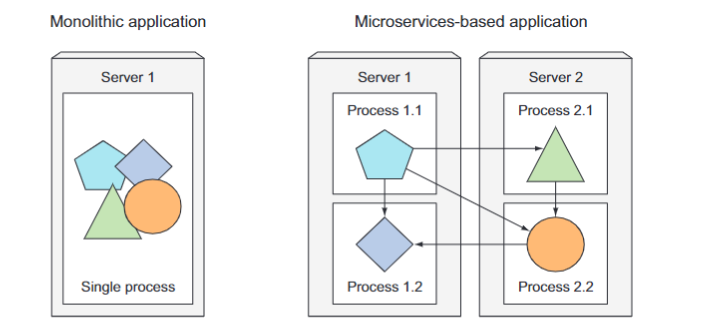
\includegraphics[width=1\textwidth]{figures/1_1.png}
		\caption{Fig. by courtesy of Marko Luksa\cite{Luksa2018}}
		\label{fig:}
	\end{figure}
}

\frame{
	\frametitle{Monolitic vs. microservices}
	\framesubtitle{}
	\begin{figure}[htbp!]
		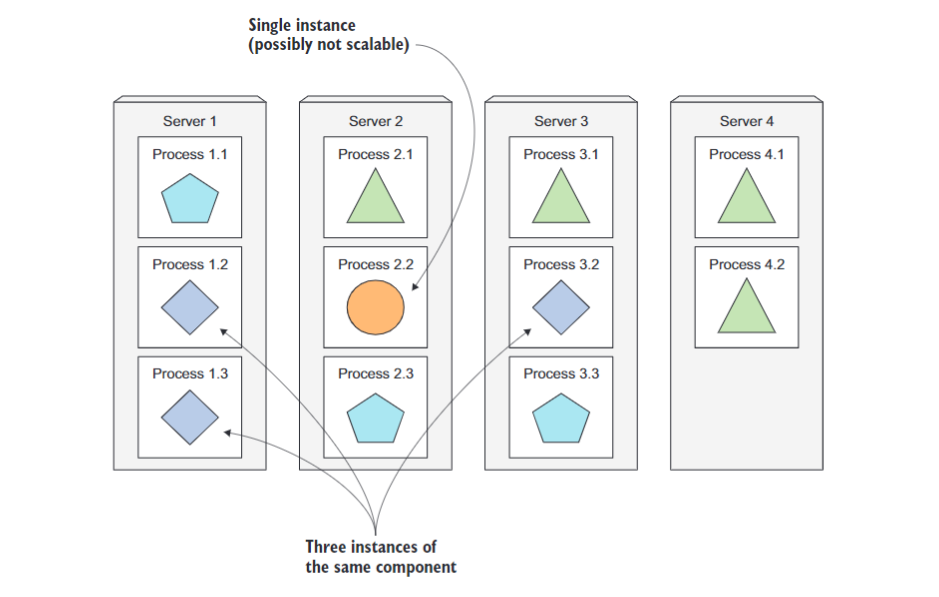
\includegraphics[width=1\textwidth]{figures/1_2.png}
		\caption{Fig. by courtesy of Marko Luksa\cite{Luksa2018}}
		\label{fig:}
	\end{figure}
}

\frame{
	\frametitle{Monolitic vs. microservices}
	\framesubtitle{}
	\begin{figure}[htbp!]
		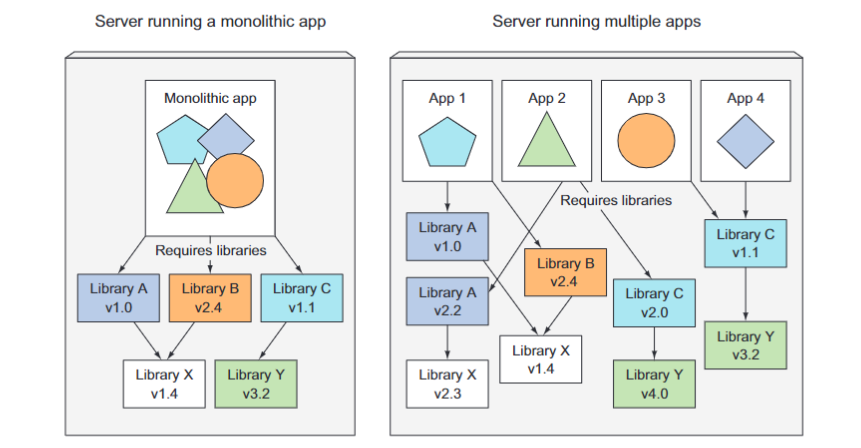
\includegraphics[width=1\textwidth]{figures/1_3.png}
		\caption{Fig. by courtesy of Marko Luksa\cite{Luksa2018}}
		\label{fig:}
	\end{figure}
}

\section[Containers]{Containers}
\frame{
	\frametitle{Containers}
	\framesubtitle{}
	Motivation
	\begin{itemize}
		\item We can't give every software component its own VM
		\item VM's are manual. We need automation
		\item Changes once place should not impact others
	\end{itemize}
	What containers are
	\begin{itemize}
		\item Containers are isolated software environments
		\item Application and dependencies bundled inside
		\item A lightweight version of VM's
	\end{itemize}
}

\frame{
	\frametitle{A normal VM vs. containers}
	\framesubtitle{}
	\begin{figure}[htbp!]
		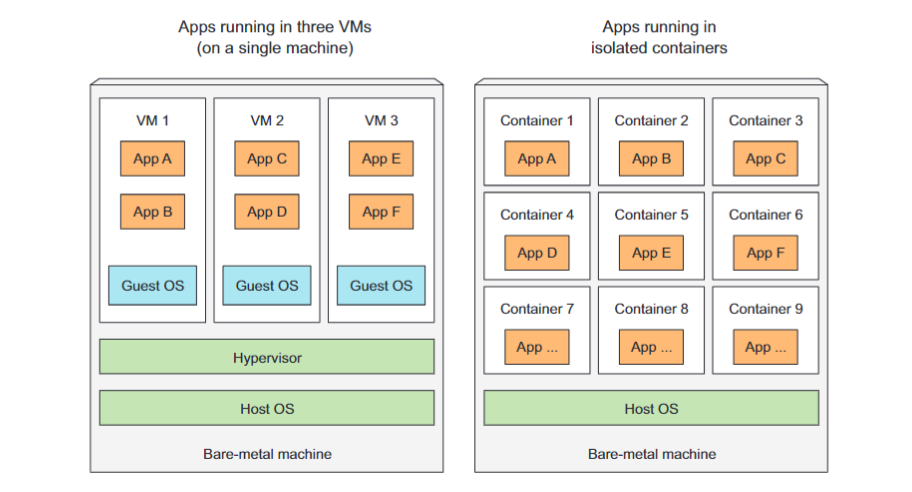
\includegraphics[width=1\textwidth]{figures/1_4.png}
		\caption{Fig. by courtesy of Marko Luksa\cite{Luksa2018}}
		\label{fig:}
	\end{figure}
}

\frame{
	\frametitle{Docker}
	\framesubtitle{}
	Motivation
	\begin{itemize}
		\item We need suitable tooling to create containers
		\item It should be automated, predictable and fast
		\item It should run everywhere, be modular and scale well
	\end{itemize}
	What Docker is
	\begin{itemize}
		\item Docker is a container tool that can run and create containers
		\item Containers only see their exact file system
		\item Similar to VM's, but less overhead
		\item Consists of reusable layers
		\item Uses a Dockerfile
	\end{itemize}
	Important concepts
	\begin{itemize}
		\item Images. Something you package your application into
		\item Registries. A repository to store your image
		\item Containers. Like normal Linux container
	\end{itemize}
}

\frame{
	\frametitle{The Docker build process}
	\framesubtitle{}
	\begin{figure}[htbp!]
		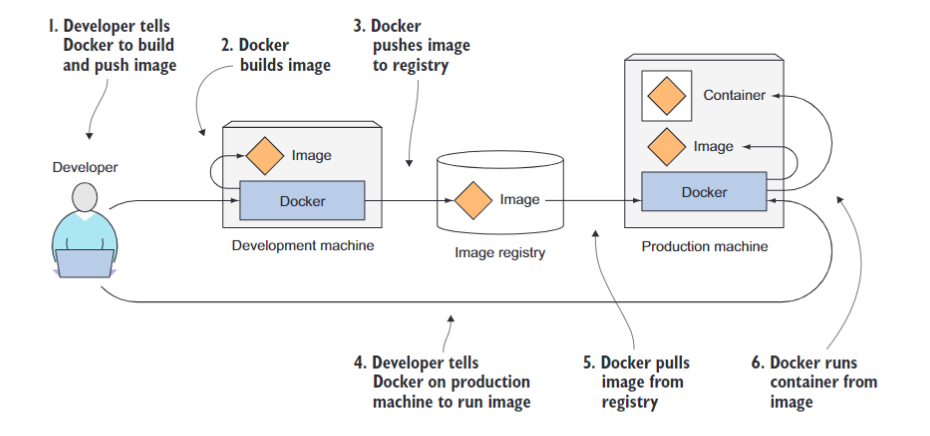
\includegraphics[width=1\textwidth]{figures/1_6.png}
		\caption{Fig. by courtesy of Marko Luksa\cite{Luksa2018}}
		\label{fig:}
	\end{figure}
}

\frame{
	\frametitle{Running apps in VM's vs. containers}
	\framesubtitle{}
	\begin{figure}[htbp!]
		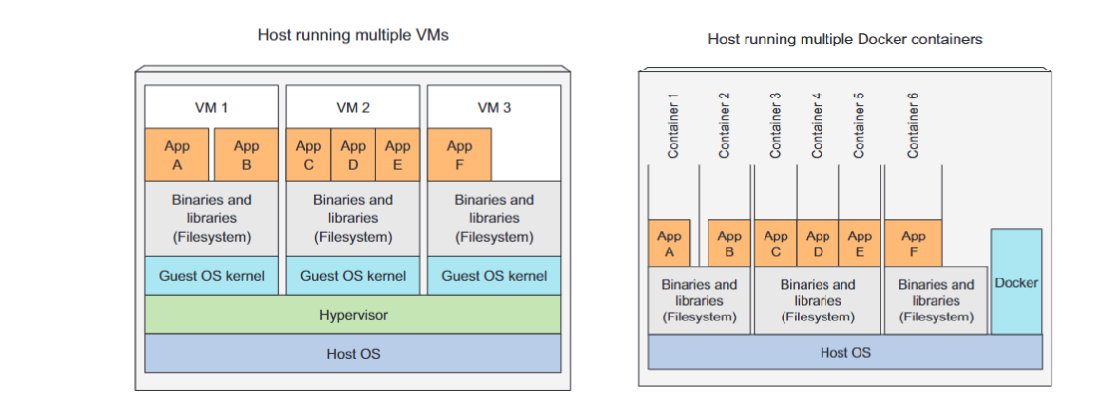
\includegraphics[width=1\textwidth]{figures/1_7.png}
		\caption{Fig. by courtesy of Marko Luksa\cite{Luksa2018}}
		\label{fig:}
	\end{figure}
}

\section[Kubernetes]{Kubernetes}
\frame{
	\frametitle{Kubernetes}
	\framesubtitle{}
	Motivation
	\begin{itemize}
		\item We need something to manage our containers
		\item Should be reliable, automated and scalable
		\item Should ease the process of deploying containers
	\end{itemize}
	What Kubernetes is
	\begin{itemize}
		\item Open-source container orchestration engine
		\item Made by Google, open-sourced in 2014
		\item Google needed to better utilize their resources
		\item Enables easy deployment, scaling and managing
		\item Exposes whole datacenter as a single platform.
	\end{itemize}
}

\frame{
	\frametitle{The Kubernetes system}
	\framesubtitle{}
	\begin{figure}[htbp!]
		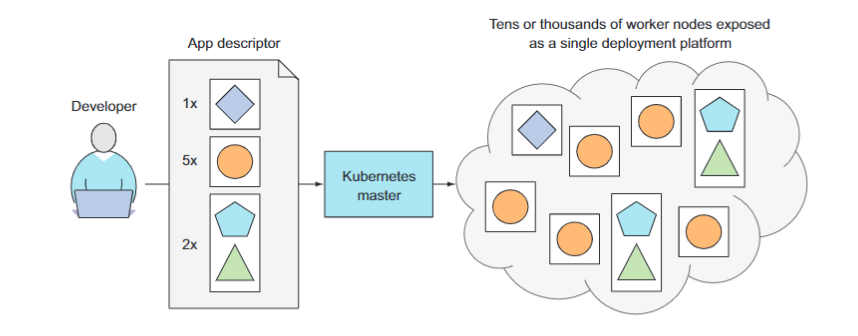
\includegraphics[width=1\textwidth]{figures/1_8.png}
		\caption{Fig. by courtesy of Marko Luksa\cite{Luksa2018}}
		\label{fig:}
	\end{figure}
}

\frame{
	\frametitle{Kubernetes cont.}
	\framesubtitle{}
	Main features of Kubernetes
	\begin{itemize}
		\item Keep containers running.
		\item Scaling copies.
		\item Hitting a moving target.
	\end{itemize}
	Benefits of using Kubernetes
	\begin{itemize}
		\item Simplifying application deployment
		\item Achieve better utilization
		\item Health checking and self-healing
		\item Automatic scaling
		\item Access to services via API/DNS
	\end{itemize}
	Enterprise-use
	\begin{itemize}
		\item Often seen as a PaaS (OpenShift)
	\end{itemize}
}

\frame{
	\frametitle{Kubernetes cont.}
	\framesubtitle{}
	The master node hosts the Control Plane and worker nodes run deployments.
	The master contains
	\begin{itemize}
		\item API Server, which you and the Control Plane components communicate with
		\item The Scheduler, which schedules your apps
		\item The Controller Manager, keeps track of workers among others
		\item etcd, a distributed db that stores cluster configuration
	\end{itemize}
	The nodes contain
	\begin{itemize}
		\item Docker, rtk or another container runtime
		\item Kubelet, which talks to the API server and manages containers
		\item Kube-proxy, which load-balances network traffic
	\end{itemize}
}

\frame{
	\frametitle{The components in Kubernetes}
	\framesubtitle{}
	\begin{figure}[htbp!]
		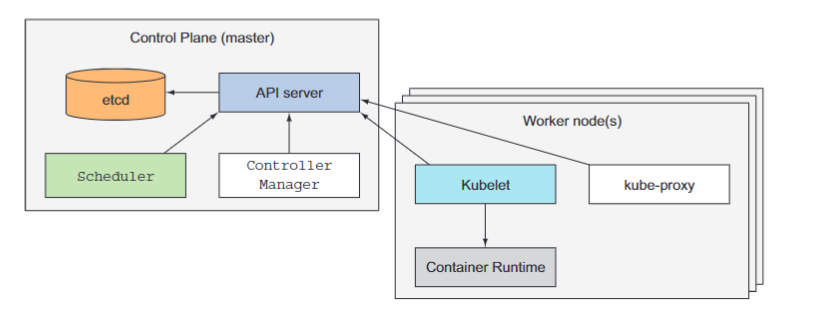
\includegraphics[width=1\textwidth]{figures/1_9.png}
		\caption{Fig. by courtesy of Marko Luksa\cite{Luksa2018}}
		\label{fig:}
	\end{figure}
}

\frame{
	\frametitle{An overview of Kubernetes's architecture}
	\framesubtitle{}
	\begin{figure}[htbp!]
		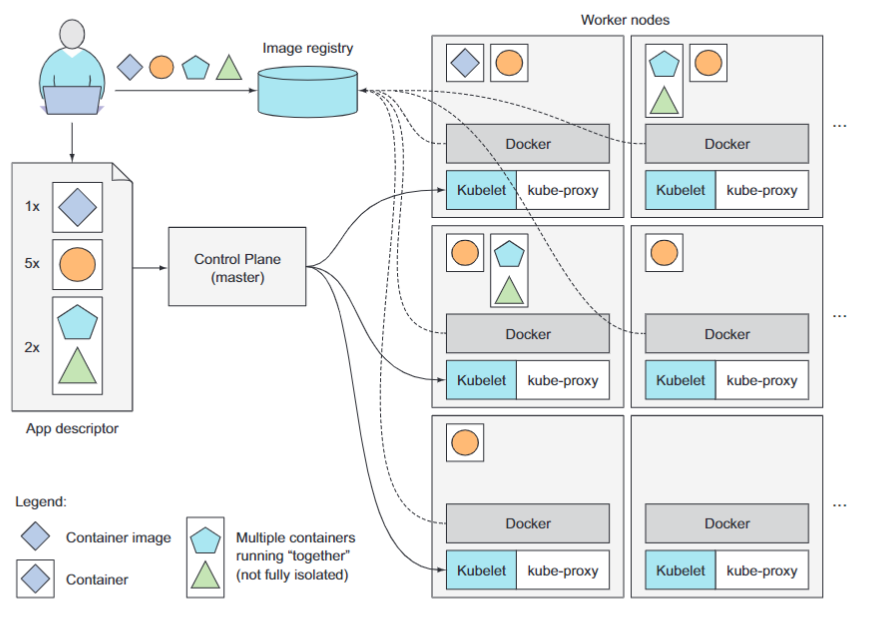
\includegraphics[width=0.8\textwidth]{figures/1_10.png}
		\caption{Fig. by courtesy of Marko Luksa\cite{Luksa2018}}
		\label{fig:}
	\end{figure}
}

\section[Hands-on]{Hands-on}
\begin{frame}[fragile]
	\frametitle{Running the busybox image}
	\framesubtitle{}
	Installing Docker and running a Hello World container
	\begin{itemize}
		\item Busybox is a single executable with many UNIX tools.
	\end{itemize}
	\begin{figure}[htbp!]
		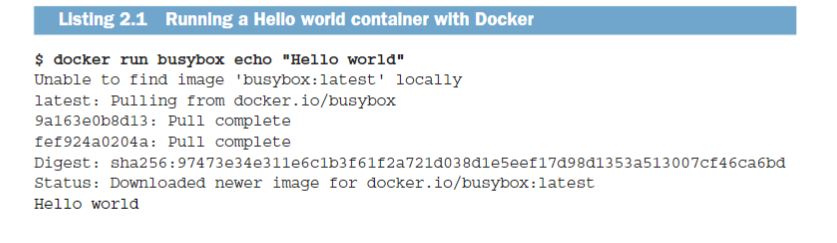
\includegraphics[width=1\textwidth]{listings/2_1.png}
		\caption{Listing. by courtesy of Marko Luksa\cite{Luksa2018}}
		\label{fig:}
	\end{figure}
	\begin{lstlisting}[numbers=none, basicstyle=\ttfamily]
$ docker run busybox echo "Hello world"
$ docker run <image>
$ docker run <image>:<tag>
	\end{lstlisting}
\end{frame}

\frame{
	\frametitle{Running echo "Hello world" in a container}
	\framesubtitle{}
	\begin{figure}[htbp!]
		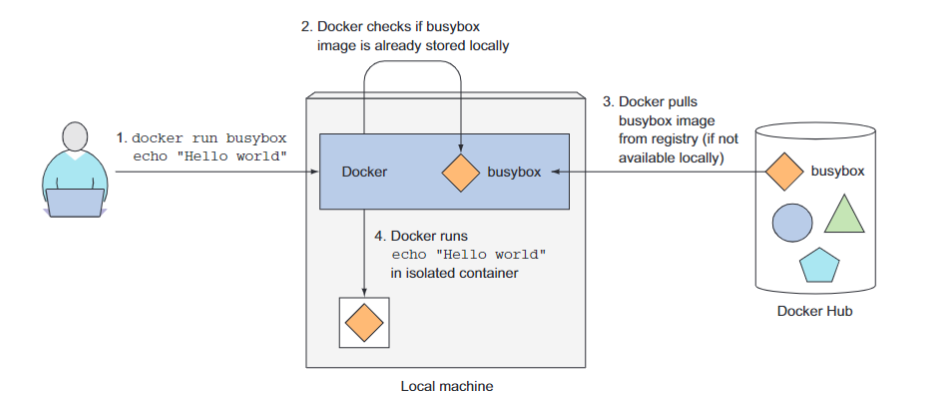
\includegraphics[width=1\textwidth]{figures/2_1.png}
		\caption{Fig. by courtesy of Marko Luksa\cite{Luksa2018}}
		\label{fig:}
	\end{figure}
}

\frame{
	\frametitle{Creating a Node.js app}
	\framesubtitle{}
	\begin{itemize}
		\item We make a simple HTTP app that can receive\\
		and reply to requests with its hostname
		\item Using Node.js and JavaScript
	\end{itemize}
	\begin{figure}[htbp!]
		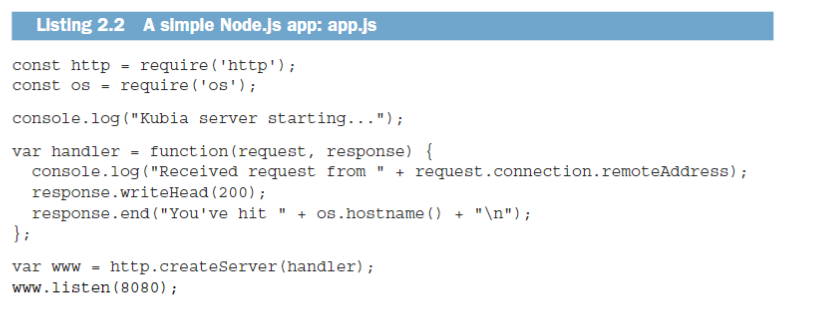
\includegraphics[width=1\textwidth]{listings/2_2.png}
		\caption{Listing. by courtesy of Marko Luksa\cite{Luksa2018}}
		\label{fig:}
	\end{figure}
}

\frame{
	\frametitle{Creating a Dockerfile for the image}
	\framesubtitle{}
	\begin{itemize}
		\item We need a Dockerfile to create an image
		\item It describes the app and its dependencies
	\end{itemize}
	\begin{figure}[htbp!]
		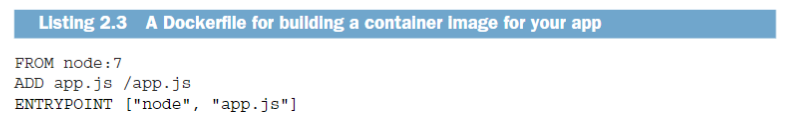
\includegraphics[width=1\textwidth]{listings/2_3.png}
		\caption{Listing. by courtesy of Marko Luksa\cite{Luksa2018}}
		\label{fig:}
	\end{figure}
}

\begin{frame}[fragile]
	\frametitle{Building the container image}
	\framesubtitle{}
	The Docker daemon builds the image.
	\begin{lstlisting}[numbers=none, basicstyle=\ttfamily]
$ docker build -t kubia .
	\end{lstlisting}
	\begin{figure}[htbp!]
		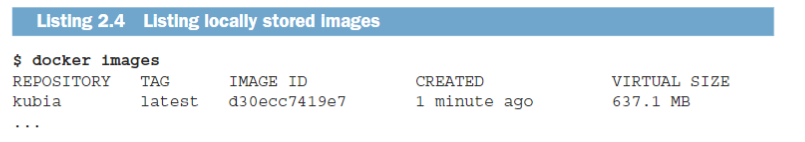
\includegraphics[width=0.9\textwidth]{listings/2_4.png}
		\caption{Listing. by courtesy of Marko Luksa\cite{Luksa2018}}
		\label{fig:}
	\end{figure}
	\begin{figure}[htbp!]
		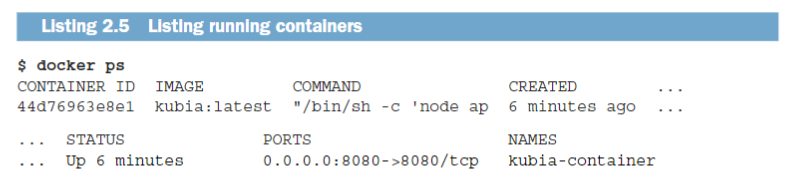
\includegraphics[width=0.9\textwidth]{listings/2_5.png}
		\caption{Listing. by courtesy of Marko Luksa\cite{Luksa2018}}
		\label{fig:}
	\end{figure}
\end{frame}

\frame{
	\frametitle{Building a new container image from a Dockerfile}
	\framesubtitle{}
	\begin{figure}[htbp!]
		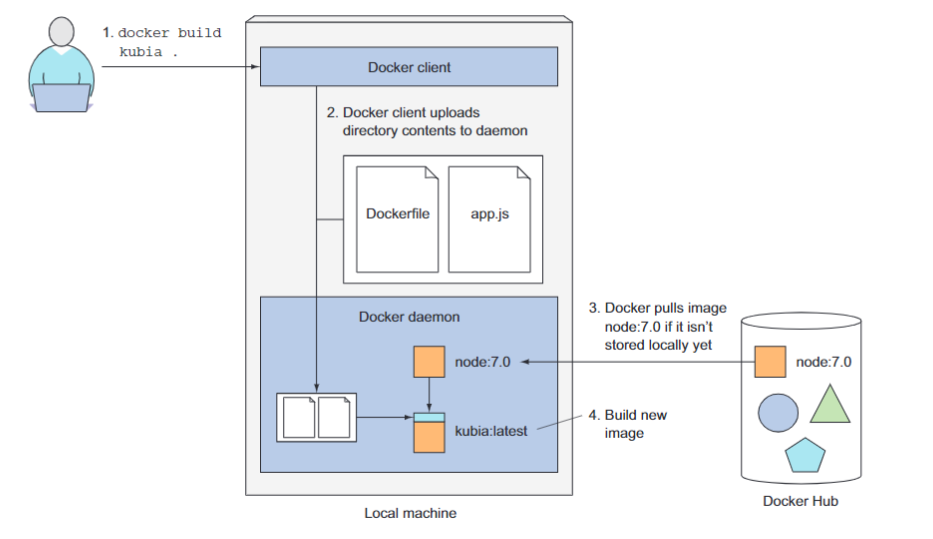
\includegraphics[width=1\textwidth]{figures/2_2.png}
		\caption{Fig. by courtesy of Marko Luksa\cite{Luksa2018}}
		\label{fig:}
	\end{figure}
}

\frame{
	\frametitle{The layers of a container image}
	\framesubtitle{}
	\begin{figure}[htbp!]
		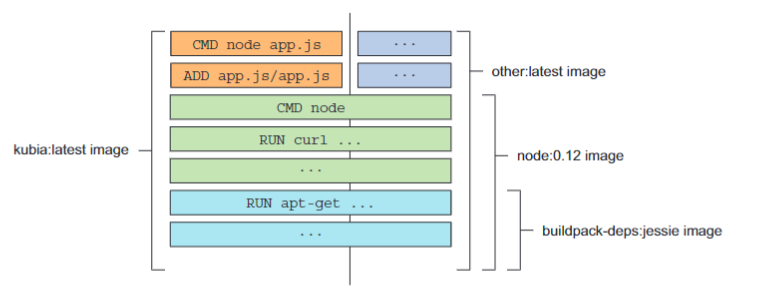
\includegraphics[width=1\textwidth]{figures/2_3.png}
		\caption{Fig. by courtesy of Marko Luksa\cite{Luksa2018}}
		\label{fig:}
	\end{figure}
}

\begin{frame}[fragile]
	\frametitle{More container commands}
	\framesubtitle{}
	Running the container image
	\begin{lstlisting}[numbers=none, basicstyle=\ttfamily]
$ docker run --name kubia-container -p 8080:8080 -d kubia
$ curl localhost:8080
	\end{lstlisting}
	Exploring the inside of a running container
	\begin{lstlisting}[numbers=none, basicstyle=\ttfamily]
$ docker exec -it kubia-container bash
$ ps aux
	\end{lstlisting}
	Stopping and removing a container
	\begin{lstlisting}[numbers=none, basicstyle=\ttfamily]
$ docker stop kubia-container
$ docker rm kubia-container
	\end{lstlisting}
\end{frame}

\frame{
	\frametitle{Output of container commands}
	\framesubtitle{}
	\begin{figure}[htbp!]
		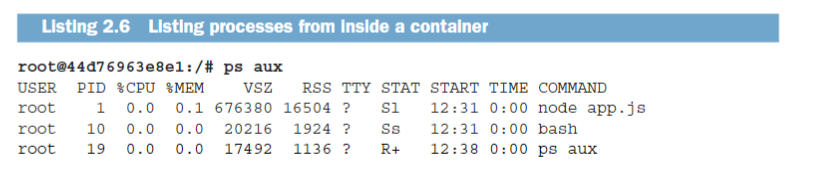
\includegraphics[width=1\textwidth]{listings/2_6.png}
		\caption{Listing. by courtesy of Marko Luksa\cite{Luksa2018}}
		\label{fig:}
	\end{figure}
	\begin{figure}[htbp!]
		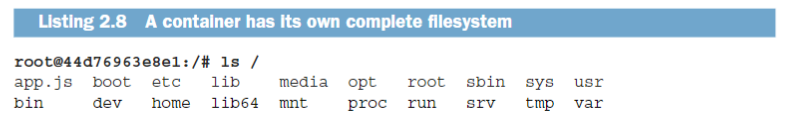
\includegraphics[width=1\textwidth]{listings/2_8.png}
		\caption{Listing. by courtesy of Marko Luksa\cite{Luksa2018}}
		\label{fig:}
	\end{figure}
}

\begin{frame}[fragile]
	\frametitle{Pushing the image to the registry}
	\framesubtitle{}
	\begin{lstlisting}[numbers=none, basicstyle=\ttfamily]
$ docker tag kubia <dockerid>/kubia
	\end{lstlisting}
	\begin{figure}[htbp!]
		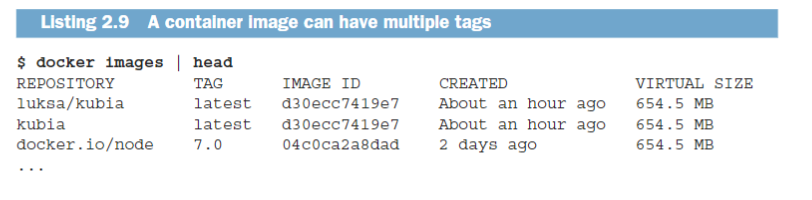
\includegraphics[width=1\textwidth]{listings/2_9.png}
		\caption{Listing. by courtesy of Marko Luksa\cite{Luksa2018}}
		\label{fig:}
	\end{figure}
	\begin{lstlisting}[numbers=none, basicstyle=\ttfamily]
$ docker push <dockerid>/kubia
$ docker run -p 8080:8080 -d <dockerid>/kubia
	\end{lstlisting}
\end{frame}

\begin{frame}[fragile]
	\frametitle{Setting up a Kubernetes cluster with Minikube}
	\framesubtitle{}
	What is minikube
	\begin{itemize}
		\item A tool that enables us to run Kubernetes locally
		\item Implements a local single node cluster
		\item Runs on macOS, Linux and Windows
		\item Used for Kubernetes development and prototyping
		\item Exercises and project make use of minikube
	\end{itemize}
	You can also order a hosted Kubernetes cluster at \\
	Google, Amazon, Microsoft Azure etc.
	\begin{lstlisting}[numbers=none, basicstyle=\ttfamily]
$ minikube start
$ kubectl get nodes
$ kubectl describe node <nodeid>
	\end{lstlisting}
\end{frame}

\frame{
	\frametitle{Introducing pods}
	\framesubtitle{}
	Before we can deploy our app, we need to know what pod is
	\begin{itemize}
		\item A pod is a group of one or more tightly\\
		related containers that run together and share\\
		the same Linux namespace
		\item Each pod is like a separate logical machine.
		\item All containers in a pod will appear to be\\
		running on the same logical machine.
	\end{itemize}
	\begin{figure}[htbp!]
		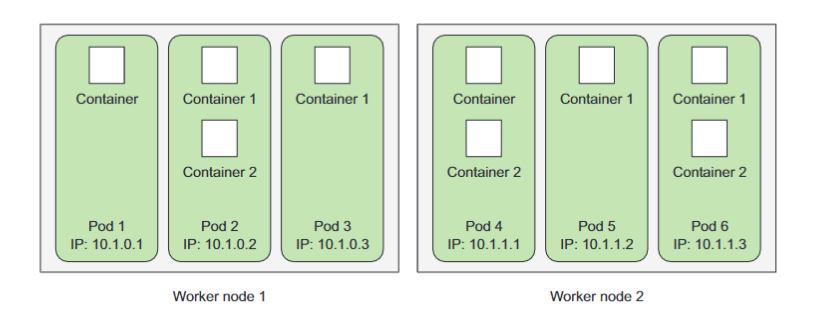
\includegraphics[width=0.8\textwidth]{figures/2_5.png}
		\caption{Fig. by courtesy of Marko Luksa\cite{Luksa2018}}
		\label{fig:}
	\end{figure}
}

\frame{
	\frametitle{Pod commands}
	\framesubtitle{}
	\begin{figure}[htbp!]
		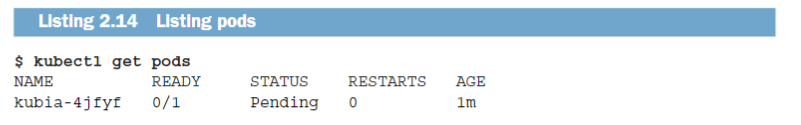
\includegraphics[width=1\textwidth]{listings/2_14.png}
		\caption{Listing. by courtesy of Marko Luksa\cite{Luksa2018}}
		\label{fig:}
	\end{figure}
	\begin{figure}[htbp!]
		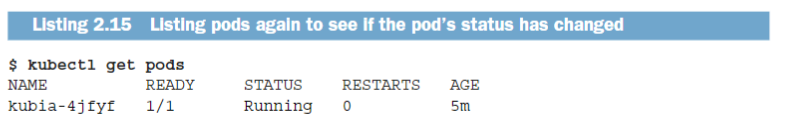
\includegraphics[width=1\textwidth]{listings/2_15.png}
		\caption{Listing. by courtesy of Marko Luksa\cite{Luksa2018}}
		\label{fig:}
	\end{figure}
}

\begin{frame}[fragile]
	\frametitle{Running our first app on Kubernetes}
	\framesubtitle{}
	\begin{lstlisting}[numbers=none, basicstyle=\ttfamily]
$ kubectl run kubia --image=<dockerid>/kubia \\
 --port=8080 --generator=run-pod/v1
pod/kubia created
	\end{lstlisting}
\end{frame}

\begin{frame}[fragile]
	\frametitle{Accessing our application}
	\framesubtitle{}
	We can create a service that exposes our pod to us
	\begin{lstlisting}[numbers=none, basicstyle=\ttfamily]
$ kubectl expose pod kubia --type=NodePort \\
 --name kubia-http
	\end{lstlisting}
	\begin{figure}[htbp!]
		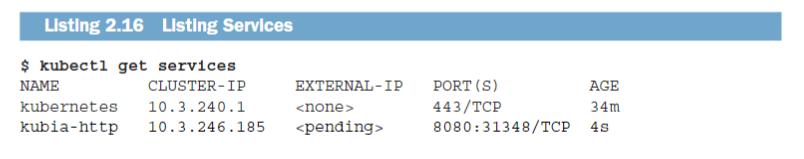
\includegraphics[width=1\textwidth]{listings/2_16.png}
		\caption{Listing. by courtesy of Marko Luksa\cite{Luksa2018}}
		\label{fig:}
	\end{figure}
\end{frame}

\frame{
	\frametitle{Accessing our application cont.}
	\framesubtitle{}
	\begin{figure}[htbp!]
		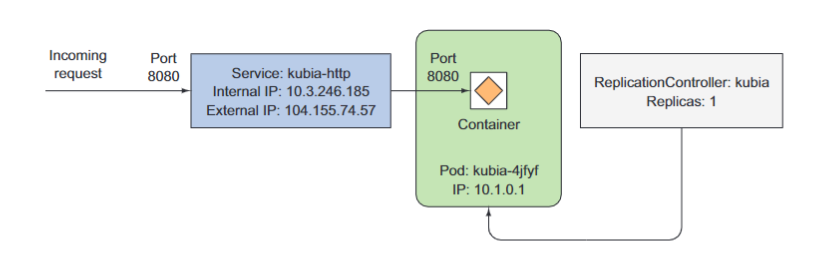
\includegraphics[width=1\textwidth]{figures/2_7.png}
		\caption{Fig. by courtesy of Marko Luksa\cite{Luksa2018}}
		\label{fig:}
	\end{figure}
}

\frame{
	\frametitle{Accessing our application cont.}
	\framesubtitle{}
	\begin{figure}[htbp!]
		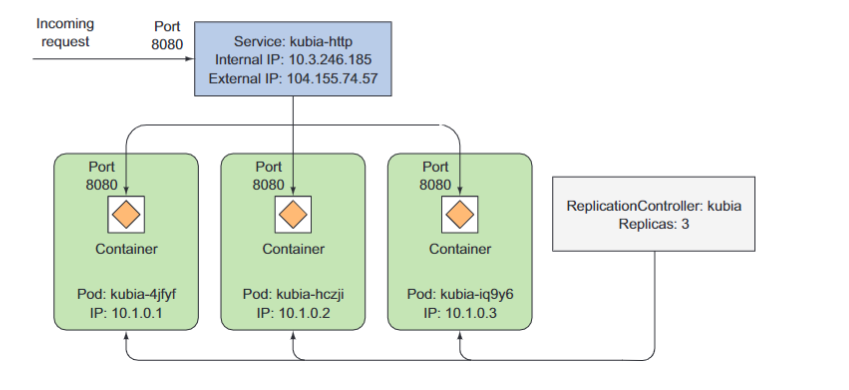
\includegraphics[width=1\textwidth]{figures/2_8.png}
		\caption{Fig. by courtesy of Marko Luksa\cite{Luksa2018}}
		\label{fig:}
	\end{figure}
}

%===============References
\begin{frame}[allowframebreaks]
\frametitle{References}
%\def\section*#1{}%remove auto heading for references
\fontsize{5pt}{5pt}\selectfont
\def\newblock{\hskip .11em plus .33em minus .07em}
\bibliographystyle{chicago}
\bibliography{cl_bibliography}
\normalsize
\end{frame}

\end{document}